\documentclass{article}
\usepackage[utf8]{inputenc}
\usepackage{graphicx}
\title{Bilan projet GL}
\author{Florentin Gonthier Germain Geoffroy Matthieu Bergeron \\ Adrien Fischman Matthias Beaupere}

\begin{document}

\maketitle

\section{Répartition des tâches et organisation de l'équipe}

\subsection{Réception du projet et mise en place des méthodes agiles}
A la réception du projet, il nous semblait essentiel que chacun comprenne le sujet dans son intégralité afin d'avoir une vision globale des tâches à effectuer. Dès lors, après une première lecture complète, nous avons pu mettre en place des méthodes Agiles.\\
Nous avons tous ensemble, sans répartition préalable, analysé les premiers éléments qui ont constitués notre premier sprint. Nous avons eu recours à Acunote, un site de management de projet agile en ligne, pour mettre en forme un premier backlog accompagné du sprint pour l'implémentation de Hello-World en définissant différentes user-stories.\\
\begin{figure}[h!]
    \centering
    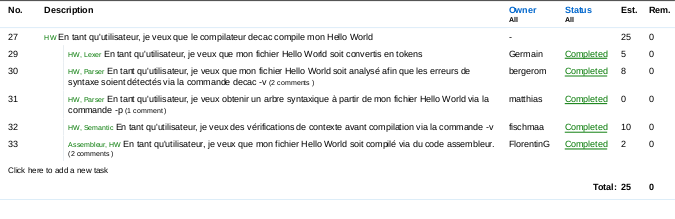
\includegraphics[scale=0.7]{sprintHelloWorld1.png}
    \caption{Sprint Hello-World, Acunote.}
    \label{fig:Sprint Hello-World}
\end{figure}
Nous avons décidé de ne pas désigner de Scrum Master. En effet, nous avons compris que la bonne communication au sein du groupe serait suffisante pour l'organisation des méthodes agiles et la répartition des tâches au cours des stand-up. \\
Ainsi, la répartition des tâches pour le premier sprint s'est fait sans difficulté : chacun a choisi de couvrir un user-story selon ses affinités avec le sujet. Matthieu et Germain se sont occupé du lexer, Matthias du parser, tandis qu'Adrien commencait l'analyse contextuelle et que Florentin se penchait sur la compilation. \\
\\

La fin de ce premier sprint a été déterminant dans le fonctionnement de notre équipe. Tous les membres de l'équipe ont fournis un travail pertinent, ce qui a instauré une confiance générale au sein du groupe. La confiance vis-à-vis du travail des autres membres de l'équipe a permis à chacun d'entre nous de se spécialiser sur un aspect en particulier du projet. Notre bonne communication permettait de s'aider mutuellement, et de demander un avis extérieur sur notre propre travail sans remise en cause de sa qualité.\\
Matthias a rejoint Adrien sur l'analyse contextuelle, Germain débutait la classe Math pendant que Matthieu et Florentin travaillait sur le langage assembleur.

\subsection{Avancement du projet et spécialisation}
Suite au rendu du sprint Hello-World, Adrien a rejoint Germain sur la classe Math. Nous avons pris la décision de nous spécialiser chacun sur une partie différentes du projet. Cette décision a été prise par le groupe tout entier, elle avait pour objectif de maximiser les compétences des membres du groupe. Chaque membre de l'équipe travaillait avec un binôme privilégié : Adrien et Germain travaillait ensemble sur la classe Math, et Matthieu assurait la liaison entre l'analyse contextuelle de Matthias et la partie assembleur de Florentin. \\
Ainsi, concrètement des sous équipes se sont distingués au sein du groupe. Ce choix de spécialisation a été permis par la confiance instaurée préalablement et nous a permis a tous de gagner en compétences pointus sur un domaine en particulier. \\
\\

La spécialisation des membres de l'équipe a impacté notre organisation agile pour le projet. La partie Math et la partie liée au compilateur étaientt dorénavant séparées. Dès lors, les sprints ne concernait plus qu'une partie à la fois. Le travail en binôme permettait une synchronisation permanente des avancées et des problèmes rencontrés, ce qui facilitait grandement la répartition des tâches futures au sein des sous équipes.

\section{Historique du projet} 
Notre projet s'est articulé autour des méthodes Agiles. Nous avons choisi d'effectuer un total de trois sprints, correspondants à des avancements importants dans le projet : 
\begin{enumerate}
    \item Le Hello World
    \item Le rendu sans-objet
    \item Le rendu final
\end{enumerate}
La partie maths, qui était indépendante du reste, ne faisait pas partie de ces sprints. \\
Lors de chaque sprint, les partie B et C étaient développées en parallèle. Notre répartition des tâches nous obligeait a avoir une communication constante entre les responsables des étapes B et C. \\
Nous avons essayé, tant que possible, d'utiliser des techniques de Test Driven Development. Les tests étaient donc écrits avant de commencer à coder une fonctionnalité. Nous nous sommes aussi efforcés de créer des binômes testeur/programmeur : sur la partie C par exemple, Matthieu a fait la plupart des tests pour le code de Florentin. \\
Une grande partie de notre travail s'est donc portée sur la validation des tests. Pour chaque étape, des scripts de validation automatique ont étés mis en place, ce qui nous a permis d'éviter d'introduire de nouveaux bugs. Cette démarche a été l'un des points forts de notre projet, puisque cela nous a permis d'avancer par incréments, et donc de gagner en agilité. C'était aussi un point positif pour le moral général de l'équipe, puisqu'on voyait notre compilateur s'améliorer de jour en jour.\\
Avec du recul, nous sommes d'accord pour dire que nous avons peut-être négligé les étapes d'analyse du projet. Cela nous a posé quelques problèmes, notamment pour la partie C qui exigeait un travail préalable sur la définition des conventions et des structures de données. \\

\section{Conclusion}
\textbf{Florentin : } \\ 
Pour la gestion du projet, je suis parti trop vite sur la partie C sans prendre assez de recul sur les éléments qui était demander. Cela s’est ressenti lors du debug de la partie C. En effet, toutes les fonctionnalités n’était pas implémentée ou complète. \\ 
Si j’avais commencé par faire un cahier des charges précis de ce à quoi devait ressembler le compilateur, je pense que le compilateur aurait été plus complet. Les opérations à faire sur la partie C n’ont pas été détaillé, et si le projet était à refaire, je ferrais cela en premier.
Sinon ce projet m’as permis d’améliorer ma compréhension de l’assembleur, même si cela restait encore de l’assembleur abstrait (à travers ima). \\ \\
\textbf{Matthieu : } \\
Le début du projet m'a paru très compliqué, puisque j'ai essayé d'avoir une vision globale du fonctionnement du compilateur. Ce choix s'est avéré payant sur le long terme, puisque j'ai réussi à naviguer entre la partie C et l'écriture de tests.\\
Si il fallait changer une chose dans notre organisation, je pense qu'on aurait du effectuer des séances de pair-programming au début des sprints. En effet cela nous aurait permis de comprendre mieux le codes des autres, et surtout de se mettre en accord sur certaines conventions. \\
A la fin du projet, j'ai compris comment fonctionnait un compilateur dans la globalité, c'était mon objectif et j'en suis très satisfait. Sachant que j'ai travaillé sur la partie C, j'ai aussi acquis une connaissance approfondie de la génération de code assembleur. 
\end{document}
